





\begin{figure}[t]
  \centering
  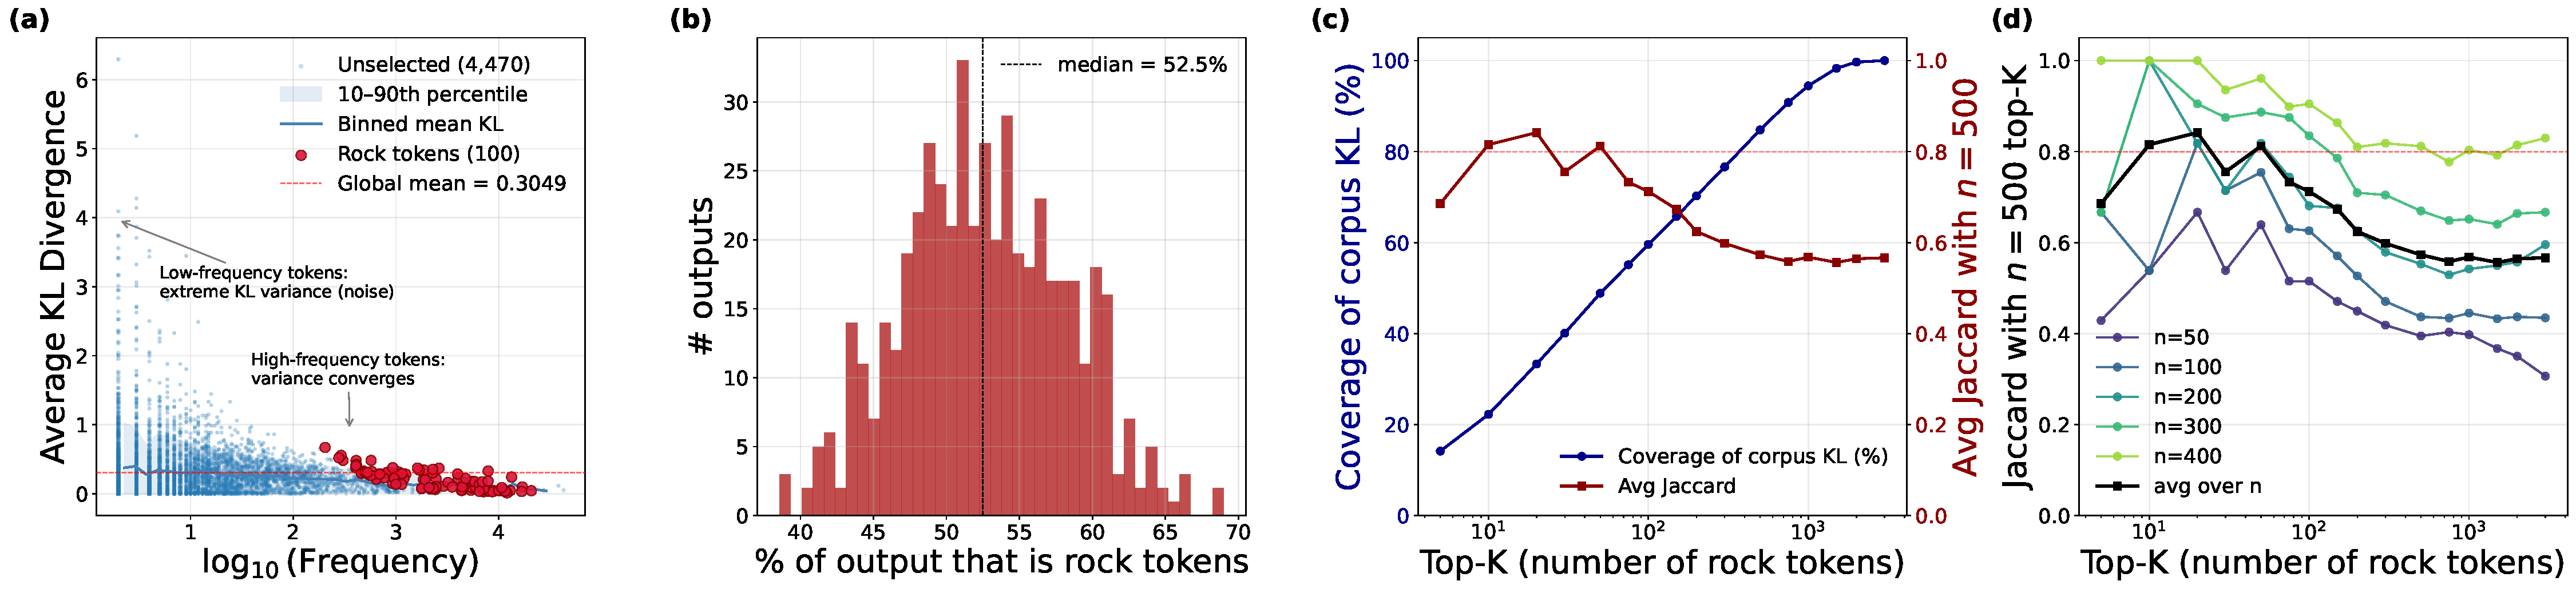
\includegraphics[width=\linewidth]{Figures/Section4/paper_figure1_combined.pdf}
  \caption{\textbf{Empirical identification and stability of Rock Tokens.}
  \textbf{(a)} Per-token KL $\widehat\ell_v$ vs.\ frequency on $N{=}500$
  MATH-500 trajectories: rare tokens are noise-dominated, while the Rock
  Score $R(v)$ isolates true Rock Tokens (red) at the upper edge of stable
  frequency bands. \textbf{(b)} Per-sequence Rock-Token density
  (median $52.5\%$). \textbf{(c)} Cumulative loss coverage (blue) and
  selection stability (red) vs.\ cutoff $K$; $K{=}100$ balances
  reproducibility with $\approx 60\%$ coverage of the distillation burden.
  \textbf{(d)} Jaccard ranking robustness across sample sizes
  $n\in[50,400]$: the top-$100$ selection is stable, larger cutoffs degrade.}

  % \caption{\textbf{Empirical identification and stability of Rock Tokens.} \textbf{(a)} Average KL Divergence ($\widehat\ell_v$) vs. token frequency ($N{=}500$ MATH-500 trajectories). Raw KL exhibits extreme small-sample variance for rare tokens. The Rock Score $R(v)$ bypasses this noise, isolating true Rock Tokens (red dots) at the upper edge of stable frequency bands. \textbf{(b)} Distribution of the percentage of Rock Tokens across generated outputs, indicating a median density of 52.5\% per sequence.\textbf{(c)} Cumulative loss coverage (blue) vs. selection stability (red) across cutoff sizes $K$. The $K{=}100$ boundary optimally balances high reproducibility with $\approx 60\%$ coverage of the total distillation burden. \textbf{(d)} Ranking robustness (Jaccard index) across sample sizes ($n{=}50$--$400$). The Top-100 selection remains highly stable before degrading at noisier cutoffs.}
  \label{fig:rock-id}
\end{figure}













\subsection{Token-Level Loss in On-Policy Distillation}
\label{sec:opd_loss}

On-policy distillation (OPD) optimizes a student policy $\pi_\theta$ by matching a teacher policy $\pi_T$ on trajectories sampled from the student's own distribution. The objective minimizes the per-token reverse KL divergence:
\begin{equation}
\mathcal{L}_{\mathrm{OPD}}(\theta) = \mathbb{E}_{x_{1:T} \sim \pi_\theta} \left[ \sum_{t=1}^{T} D_{\mathrm{KL}} \left( \pi_\theta(\cdot | x_{<t}) \| \pi_T(\cdot | x_{<t}) \right) \right].
\end{equation}
The loss at position $t$ is $\ell_t = \log \pi_\theta(x_t | x_{<t}) - \log \pi_T(x_t | x_{<t})$, measuring the student-teacher mismatch~\cite{fu2026revisiting}. Ideally, as the student aligns with the teacher, the magnitude of $\ell_t$ should systematically diminish across the vocabulary, leading to an optimization plateau where corrective signals eventually vanish.

\subsection{Defining and Detecting Rock Tokens}
\label{sec:rock_tokens}

Contrary to the expected convergence, we observe a subset of tokens that persistently exhibit high KL divergence even after training saturation. We term these \textbf{Rock Tokens}. 

At an intuitive level, our detection method isolates these tokens based on their \textit{Total Distillation Burden}—the absolute volume of optimization capacity consumed by a specific vocabulary item across the entire training corpus. Since the loss $\mathcal{L}_{\mathrm{OPD}}$ is an expectation over student trajectories, it admits an exact additive decomposition over token types $v$ in the vocabulary $\mathcal{V}$:
\begin{equation}
\mathcal{L}_{\text{OPD}}(\theta) = \mathbb{E}_{x \sim \pi_\theta} \left[ \sum_{t} \ell_t \right] = \sum_{v \in \mathcal{V}} \underbrace{\text{Freq}(v) \cdot \mathbb{E}[\ell_t \mid x_t = v]}_{R(v)}
\end{equation}

We formally define the \textbf{Rock Score} as $R(v) = \bar{\ell}_v \cdot \mathrm{Freq}(v)$, where $\bar{\ell}_v$ is the empirically estimated mean KL loss of token $v$ at the final checkpoint. The Rock Score $R(v)$ is therefore not an approximation, but the exact contribution of token type $v$ to the total loss that OPD minimizes. Ranking tokens by $R(v)$ is the unique additive ranking that strictly agrees with the OPD objective.

The $\mathrm{Freq}(v)$ factor acts as a natural regularizer: it up-weights tokens whose mean-loss estimate converges quickly under heavy sampling, while heavily discounting rare tokens whose mean is dominated by small-sample variance. Detection via $R(v)$ thus simultaneously aligns with the theoretical training objective while remaining robust to the empirical estimation noise inherent in natural language generation. 

Operationally, $R(v)$ prioritizes tokens that exhibit both a substantial occurrence count and an above-baseline per-token loss. Rare tokens with extreme observed losses receive appropriately low scores because their $\mathrm{Freq}(v)$ weight is minimal. As demonstrated empirically in Figure~\ref{fig:rock-id}, the top-ranked tokens cluster in the mid-to-high frequency range and sit at the upper edge of the loss distribution within their respective frequency bands, successfully filtering out the rare-but-extreme statistical outliers.








\subsection{Empirical Analysis}
\label{sec:rock_empirical}
Rock tokens exhibit persistently high expected KL divergence between student $\pi_\theta$ and teacher $\pi_T$ after on-policy distillation. We estimate this per-token loss $\widehat\ell_v = \widehat{\mathbb{E}}\big[D_{\mathrm{KL}}\!\big(\pi_\theta(\cdot \mid x_{<t}) \;\|\; \pi_T(\cdot \mid x_{<t})\big) \mid x_t = v\big]$ using student rollouts.

\textbf{Setup} The student (Qwen3-4B-Instruct) is on-policy distilled from the teacher (Qwen3-30B-A3B-Instruct) using OpenThoughts. Per-token KL is sampled from OpenThoughts and evaluated on $N{=}500$ MATH-500 problems (full details in Section~\ref{setup}).

\textbf{Observations} Figure~\ref{fig:rock-id} illustrates the distribution and density of the identified Rock Tokens within the student's generated trajectories. Panel (a) displays the absolute count of Rock Tokens per sequence, while Panel (b) normalizes this count as a percentage of the total sequence length. Strikingly, the data reveals that Rock Tokens are highly concentrated, comprising a median of 52.5\% of the total tokens in every generated output.

\begin{takeaway}
\textcolor{tabblue}{\textbf{Take-away}}~ \textbf{The Pervasiveness of Rock Tokens:} Although Rock Tokens represent a tightly constrained subset of the overall vocabulary (e.g., $K=100$), their footprint during generation is massive. Over half of the model's reasoning trajectory consists of these stubborn structural and formatting tokens, demonstrating that the primary locus of student-teacher disagreement occurs consistently throughout the core scaffolding of the output.
\end{takeaway}


\subsection{Determining the Rock Token Cutoff}\label{sec:cutoff_selection}Defining the boundary of the Rock Token set $\mathcal{R}$ requires choosing a cutoff $K$ that balances \textit{selection stability} (reproducibility across samples) against \textit{loss coverage} (fraction of optimization loss captured). A small $K$ yields a stable set but low coverage, while a large $K$ captures more loss but degrades under sampling noise.

Empirical sweeps (Figures 1b and 1c) identify an optimal intersection at $K=100$. This boundary accounts for roughly 60\% of the corpus-level KL divergence while maintaining high stability across subset sizes. We therefore adopt $K=100$ to ensure a mathematically reproducible vocabulary for subsequent analyses. Comprehensive stability metrics and sweeping procedures are detailed in Appendix \ref{app:rock_ratio}.


% \textbf{Results} Figure~\ref{fig:rock-id}(b) plots Jaccard against $K$, with one curve per $n$ and an averaged curve. Average Jaccard exceeds $0.70$ for $K \leq 100$ and decays toward a $\approx 0.57$ floor for $K \geq 150$ — beyond which the additional tokens are no longer reliably reproduced across sub-corpora. Figure~\ref{fig:rock-id}(c) overlays the corresponding coverage curve: at $K = 100$, $\mathcal{R}$ accounts for $\approx 60\%$ of the corpus-level KL while remaining within the stable regime. We therefore set $K = 100$ ($\approx 2.5\%$ of the observed vocabulary) for the remainder of the paper. This choice represents an explicit tradeoff: $K = 50$ would yield modestly higher stability ($J \approx 0.81$) but reduce coverage to $\approx 49\%$.




\begin{figure*}[t]
  \centering
  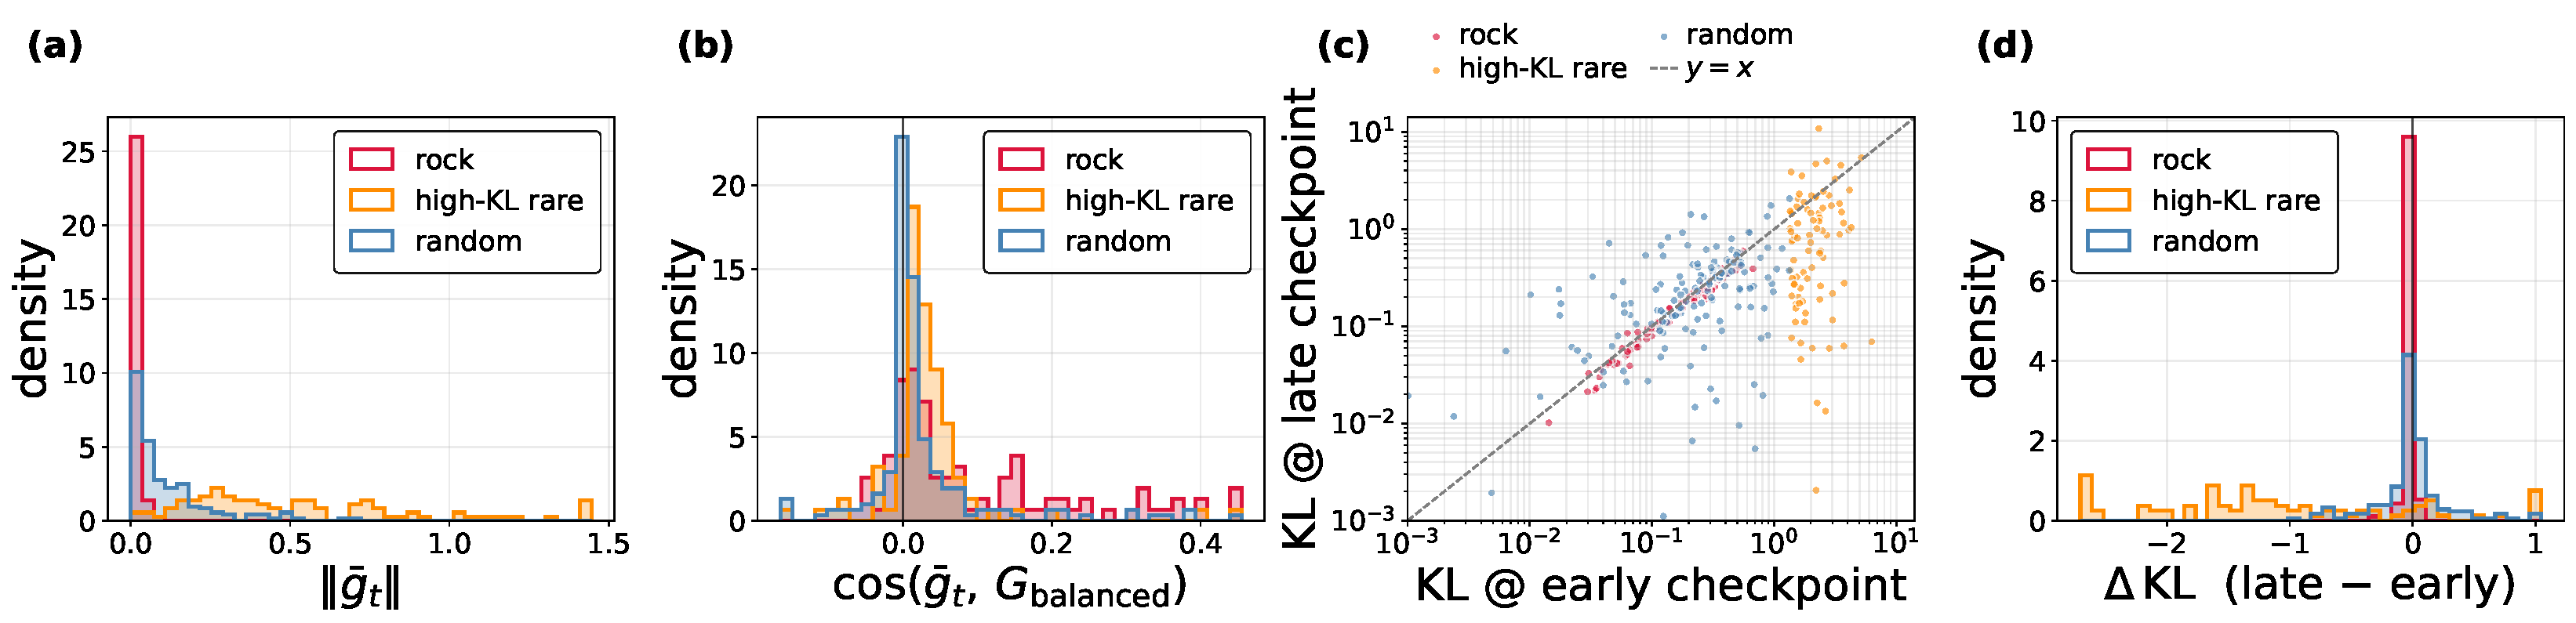
\includegraphics[width=\textwidth]{Figures/Section4/paper_figure2_gradient.pdf}
  \caption{\textbf{Per-token gradient geometry and persistence under
  training.}
  (a) Per-token logit-gradient magnitude $\|\bar{g}_{t}\|$ by group: rocks
  are an order of magnitude smaller than rare high-KL tokens.
  (b) Cosine alignment with the frequency-balanced descent direction
  $G_{\mathrm{balanced}}$: rocks are positively aligned, with a tail
  reaching $\cos > 0.3$.
  (c) Per-token mean KL paired across two training checkpoints (log-log).
  Points below the diagonal indicate KL reduction during further training;
  rocks lie on the diagonal, rare high-KL tokens fall below.
  (d) Distribution of $\Delta\mathrm{KL} = \mathrm{KL}_{\mathrm{late}} -
  \mathrm{KL}_{\mathrm{early}}$ by group: rocks concentrate at
  $\Delta\mathrm{KL} \approx 0$ (persistent); rare high-KL tokens have
  large negative $\Delta\mathrm{KL}$ (learned).}
  \label{fig:gradient}
\end{figure*}


\subsection{Analysis of Rock Tokens}

We decoded the top-$K{=}100$ Rock Tokens into their string forms using the Qwen3 tokenizer. Despite being identified by a purely numerical criterion, the resulting set is functionally coherent: Rock Tokens consistently mark structural or discourse boundaries in mathematical reasoning. 

As detailed in Appendix~\ref{analysis_rock}, four functional clusters dominate $\mathcal{R}$: (1) \textbf{LaTeX and math delimiters}, (2) \textbf{Markdown and whitespace structure}, (3) \textbf{Discourse markers} (e.g., ``So'', ``Wait''), and (4) \textbf{Digits}. In contrast, frequency-matched controls ($\mathcal{S}_{\text{ctrl}}$) predominantly consist of content-bearing tokens (e.g., nouns, verbs) used at non-boundary positions.

\begin{takeaway}
\textcolor{tabblue}{\textbf{Take-away}}~ \textbf{Structure Over Content:} The clustering of $\mathcal{R}$ at boundaries indicates student-teacher divergence centers on \textbf{how to structure} reasoning rather than \textbf{what content} to generate. Rock Tokens are a signature of the on-policy regime, marking where the student systematically resists the teacher's discourse style.
\end{takeaway}



% \subsection{Empirical Observations on Gradient Geometry and Persistence}

% Having established that Rock Tokens primarily comprise syntactic and structural scaffolding, we address \textbf{RQ1: Do Rock Tokens still provide useful learning signals during optimization?} To determine whether their persistent high loss effectively translates into steady directional guidance or merely stagnant optimization noise, we characterize their training dynamics and geometric properties through a comparative analysis against rare high-KL tokens and random tokens (illustrated in Figure~\ref{fig:gradient}). A formal mathematical decomposition of the per-token gradient contributions, alongside complete statistical significance testing, is detailed in Appendix \ref{app:gradient_geometry}. Our findings are summarized as follows:

% \textbf{Low Gradient Magnitude vs. High Frequency (Panel a):} 
%     Rock Tokens are characterized by significantly lower individual logit-gradient magnitudes ($\|\bar{g}_t\|$) compared to standard learnable high-loss tokens. However, because of their massive frequency in the training corpus, this small per-occurrence signal accumulates into a dominant aggregate force on the weight updates.

% \textbf{Alignment with Global Optimization (Panel b):} 
%     Counter-intuitively, the gradient direction of Rock Tokens ($\bar{g}_t$) exhibits a higher cosine similarity with the balanced global gradient ($G_{\text{balanced}}$) than other groups. This suggests that, from the teacher's perspective, Rock Tokens do indeed point toward a "correct" optimization path for the overall objective.

% \textbf{Persistence During Training (Panel c):} 
%     By comparing KL divergence at early versus late checkpoints, we observe that learnable high-KL tokens move significantly below the $y=x$ diagonal, indicating successful optimization. In contrast, Rock Tokens and random tokens cluster closely along the diagonal, demonstrating their resistance to training signals.

% \textbf{Optimization Stagnation (Panel d):} 
%     The distribution of $\Delta \text{KL}$ confirms that Rock Tokens remain largely "untrained," with their change in loss concentrated sharply at zero. While major high-loss tokens show a significant decrease in KL, random tokens exhibit a symmetric, noisy distribution, further highlighting the unique stagnation of Rock Tokens.

% \begin{takeaway}
% \textcolor{tabblue}{\textbf{Take-away}}~ \textbf{The Gradient Paradox:} Rock Tokens \textit{do} provide useful learning signals, generating gradients that are well-aligned with the global optimization target (Panel b). However, they remain stagnant and "untrained" throughout the OPD process (Panel d). This paradox suggests that their persistence is not due to a lack of constructive signal, but rather the student model's internal optimization bias, which stubbornly prioritizes pre-existing structural scaffolding over the teacher's stylistic direction.
% \end{takeaway}




\subsection{Empirical Observations on Gradient Geometry and Persistence}

Having established that Rock Tokens primarily comprise syntactic and structural scaffolding, we address \textbf{RQ1: Do Rock Tokens still provide useful learning signals during optimization?} To determine whether their persistent high loss effectively translates into steady directional guidance or merely stagnant optimization noise, we characterize their training dynamics and geometric properties against rare high-KL tokens and random tokens (illustrated in Figure~\ref{fig:gradient}). 

To formally evaluate this, we analyze the geometry of per-token gradients. For each token type $t$ with $n_{t}$ occurrences, we compute the mean per-occurrence reverse-KL gradient in logit space, $\bar{g}_{t} = \tfrac{1}{n_{t}} \sum_{i} g_{i}$. We then decompose its contribution to the global descent as:
\begin{equation}
\mathrm{contrib}(t) \;=\; n_{t} \,\cdot\, \|\bar{g}_{t}\| \,\cdot\, \cos\bigl(\bar{g}_{t},\, G_{\mathrm{balanced}}\bigr),
\label{eq:contrib}
\end{equation}
where $G_{\mathrm{balanced}} = \sum_{t} \bar{g}_{t}$ is a frequency-balanced reference that grants every token type equal weight, deliberately removing the trivial frequency-weighted dominance of common tokens. This decomposition yields several key insights corresponding to our empirical observations:

\textbf{Low Gradient Magnitude vs. High Frequency (Panel a):} 
Rock tokens are characterized by substantially \emph{smaller} per-occurrence gradient magnitudes than rare high-KL tokens (median $\|\bar{g}_{t}\| \approx 0.016$ versus $\approx 0.54$; Mann-Whitney $p < 10^{-30}$). However, the multiplicative decomposition in Eq.~\ref{eq:contrib} shows that rock dominance arises from the \emph{frequency} factor ($n_t$): because of their massive occurrence rate in the training corpus, this small per-token signal accumulates into a dominant aggregate force on the weight updates.

\textbf{Alignment with Global Optimization (Panel b):} 
Counter-intuitively, the gradient direction of Rock Tokens ($\bar{g}_t$) exhibits non-trivially positive directional alignment with the balanced global gradient $G_{\mathrm{balanced}}$ (median $\cos \approx 0.040$ versus $\approx 0.025$ for high-KL and $\approx 0.006$ for random tokens), with a sub-population reaching $\cos > 0.3$. This means that each rock contributes a small but consistently aligned signal at many positions, whereas rare high-KL tokens contribute large but direction-distinct signals at very few. From the teacher's perspective, Rock Tokens do indeed point toward a ``correct'' optimization path for the overall objective.

\textbf{Persistence During Training (Panel c \& d):} 
To confirm that this directional alignment translates into resistance to further learning, we compare per-token KL between an early and late checkpoint. Rare high-KL tokens experience a substantial reduction in KL (median $2.02 \to 0.85$, $\sim 58\%$; Wilcoxon $p < 10^{-8}$), moving significantly below the $y=x$ diagonal. In contrast, Rock Tokens remain essentially unchanged (median $0.21 \to 0.19$), clustering sharply along the diagonal with the distribution of $\Delta \text{KL}$ concentrated exactly at zero (Panel d). Random control tokens show a symmetric, noisy distribution with no net change.

This optimization stagnation is geometrically consistent with our gradient findings: rare high-KL tokens possess direction-distinct gradients that focused updates can isolate and resolve. Conversely, because rocks contribute highly aligned gradients, their targeted reduction would be indistinguishable from following the global descent. Thus, they receive no separable, token-specific learning signal to overcome their inherent loss.


While our gradient decomposition explains the geometry of this stagnation, the underlying mechanical cause remains open. We hypothesize this paradox is driven by adaptive optimizers under heavy-tailed class imbalance~\cite{kunstner2024heavytailedclassimbalanceadam}. Unlike in pre-training—where Adam beneficially suppresses frequent tokens to avoid overfitting structural noise—On-Policy Distillation often requires updating these exact high-frequency structural tokens to match a teacher's formatting or style. By inflating the second-moment estimates for ubiquitous Rock Tokens, Adam systematically neutralizes their effective learning rate, trapping the student in pre-existing habits despite possessing accurate directional gradients. We leave the formal verification of this optimizer-suppression hypothesis to future work.

\begin{takeaway}
\textcolor{tabblue}{\textbf{Take-away}}~ \textbf{The Gradient Paradox:} Rock Tokens \textit{do} provide useful learning signals, generating gradients that are well-aligned with the global optimization target (Panel b). However, they remain stagnant and "untrained" throughout the OPD process (Panel d). This paradox suggests that their persistence is not due to a lack of constructive signal, but rather the student model's internal optimization bias, which stubbornly prioritizes pre-existing structural scaffolding over the teacher's stylistic direction because the rock-token signal is mathematically inseparable from the global descent direction.
\end{takeaway}